\documentclass[a4paper,12pt]{article} 
\usepackage [utf8x] {inputenc}
\usepackage [T2A] {fontenc}
\usepackage [english, russian] {babel}	
\usepackage{amsmath,amsfonts,amssymb,amsthm,mathtools} 
\usepackage[colorlinks, linkcolor = blue]{hyperref}
\usepackage{upgreek}\usepackage[left=2cm,right=2cm,top=2cm,bottom=3cm,bindingoffset=0cm]{geometry}
\usepackage{graphicx}
\usepackage{subfig}
\usepackage{xcolor}
\usepackage{placeins}



\title{Лабораторная работа 3.6.1:\\Спектральный анализ электрических сигналов}
\author{Дроздов Т. А.\\Кириллов М. А.\\Б03-202}
\date{}


\begin{document}
\maketitle

\textbf{В работе используются}: генератор сигналов произвольной формы, цифровой осциллограф с функцией быстрого преобразования Фурье или цифровой USB-осциллограф, подключённый к персональному компьютеру.


\textbf{Цель работы}: 
изучить спектры сигналов различной формы и влияние параметров сигнала
на вид соответствующих спектров; проверить справедливость соотношений неопределённостей; познакомиться с работой спектральных фильтров на примере RC-цепочки.



\section*{Ход работы}
 \subsection*{Исследование спектра периодической последовательности прямоугольных импульсов и проверка соотношений неопределённостей}
Следуя техническому описанию генератора мы настроили генерацию прямоугольных импульсов с параметрами $\nu_{\text{повт}} = 1$ кГц и длительностью импульса $\tau = 50$ мкс.

Получили на экране спектр сигнала и, изменяя либо $\tau$, либо $\nu_{\text{повт}}$, наблюдали, как изменяется спектр.
\begin{figure}
    \centering
    \subfloat[$\nu_{\text{повт}} = 1$ кГц, $\tau = 10$ мкс.]{{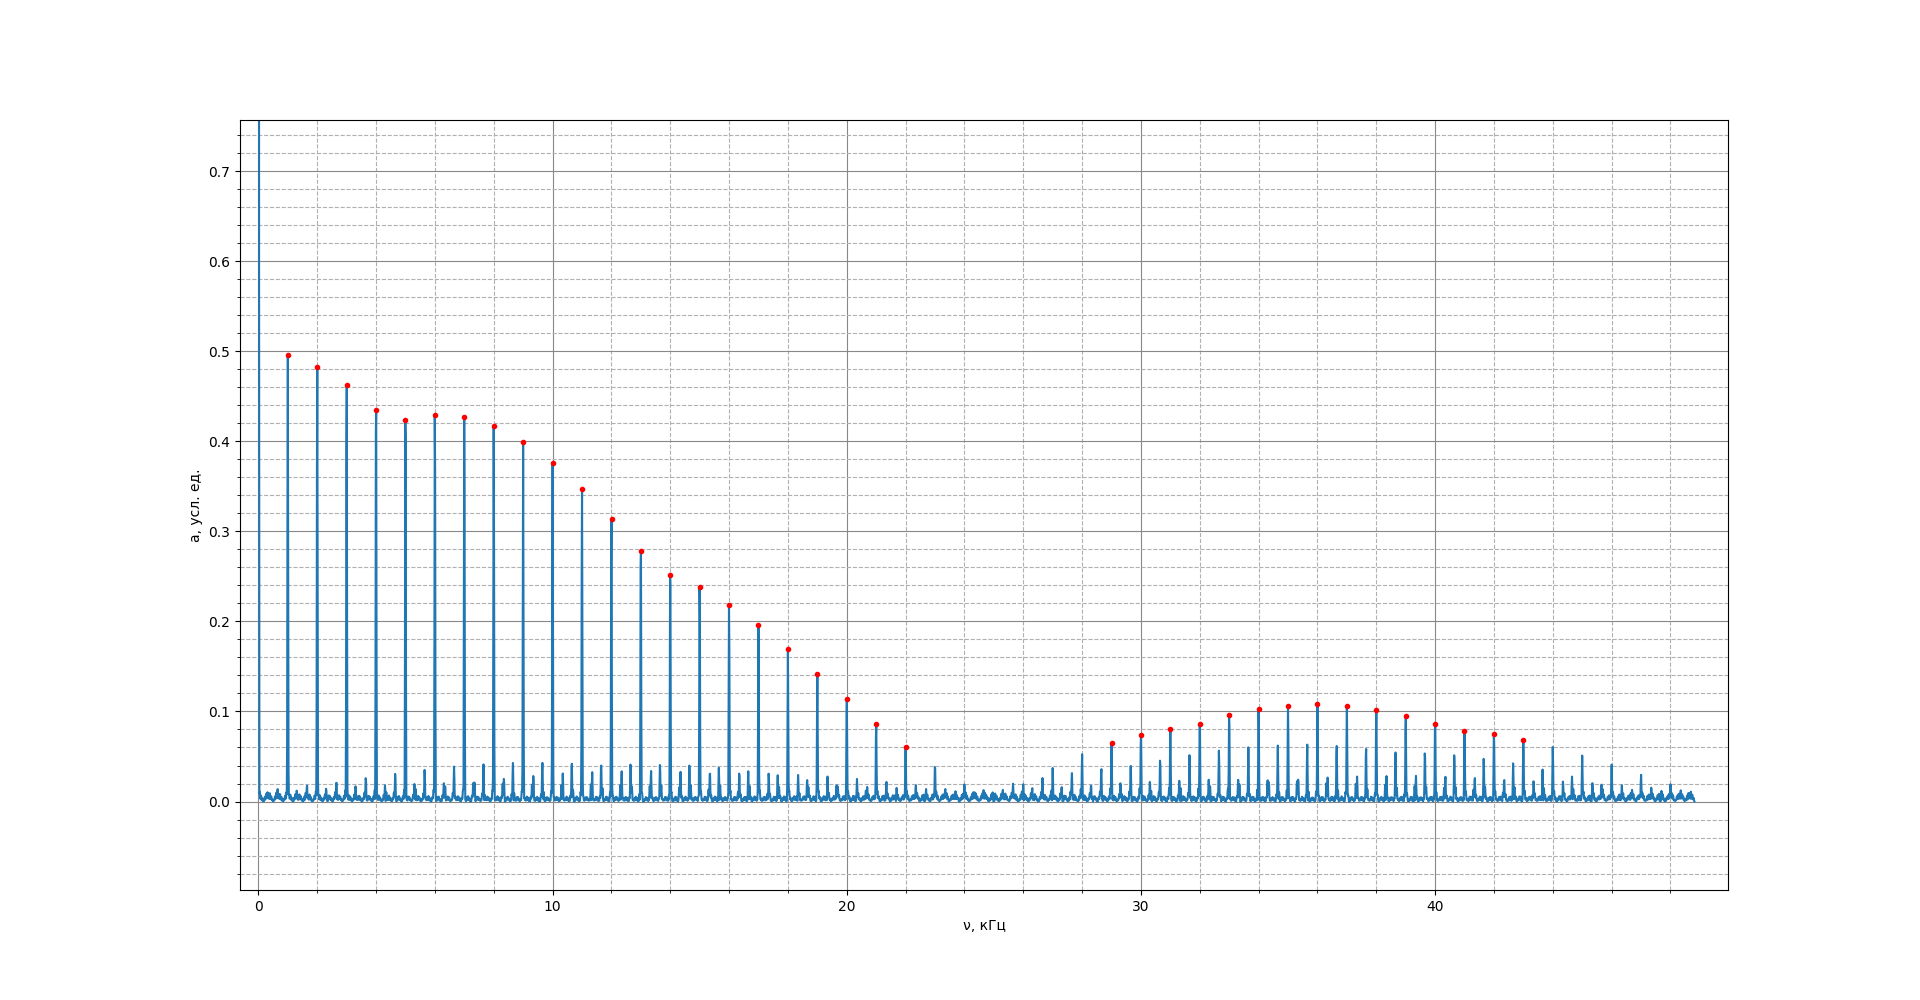
\includegraphics[width=0.5\textwidth]{10us.png}}}
    \subfloat[$\nu_{\text{повт}} = 1$ кГц, $\tau = 20$ мкс.]{{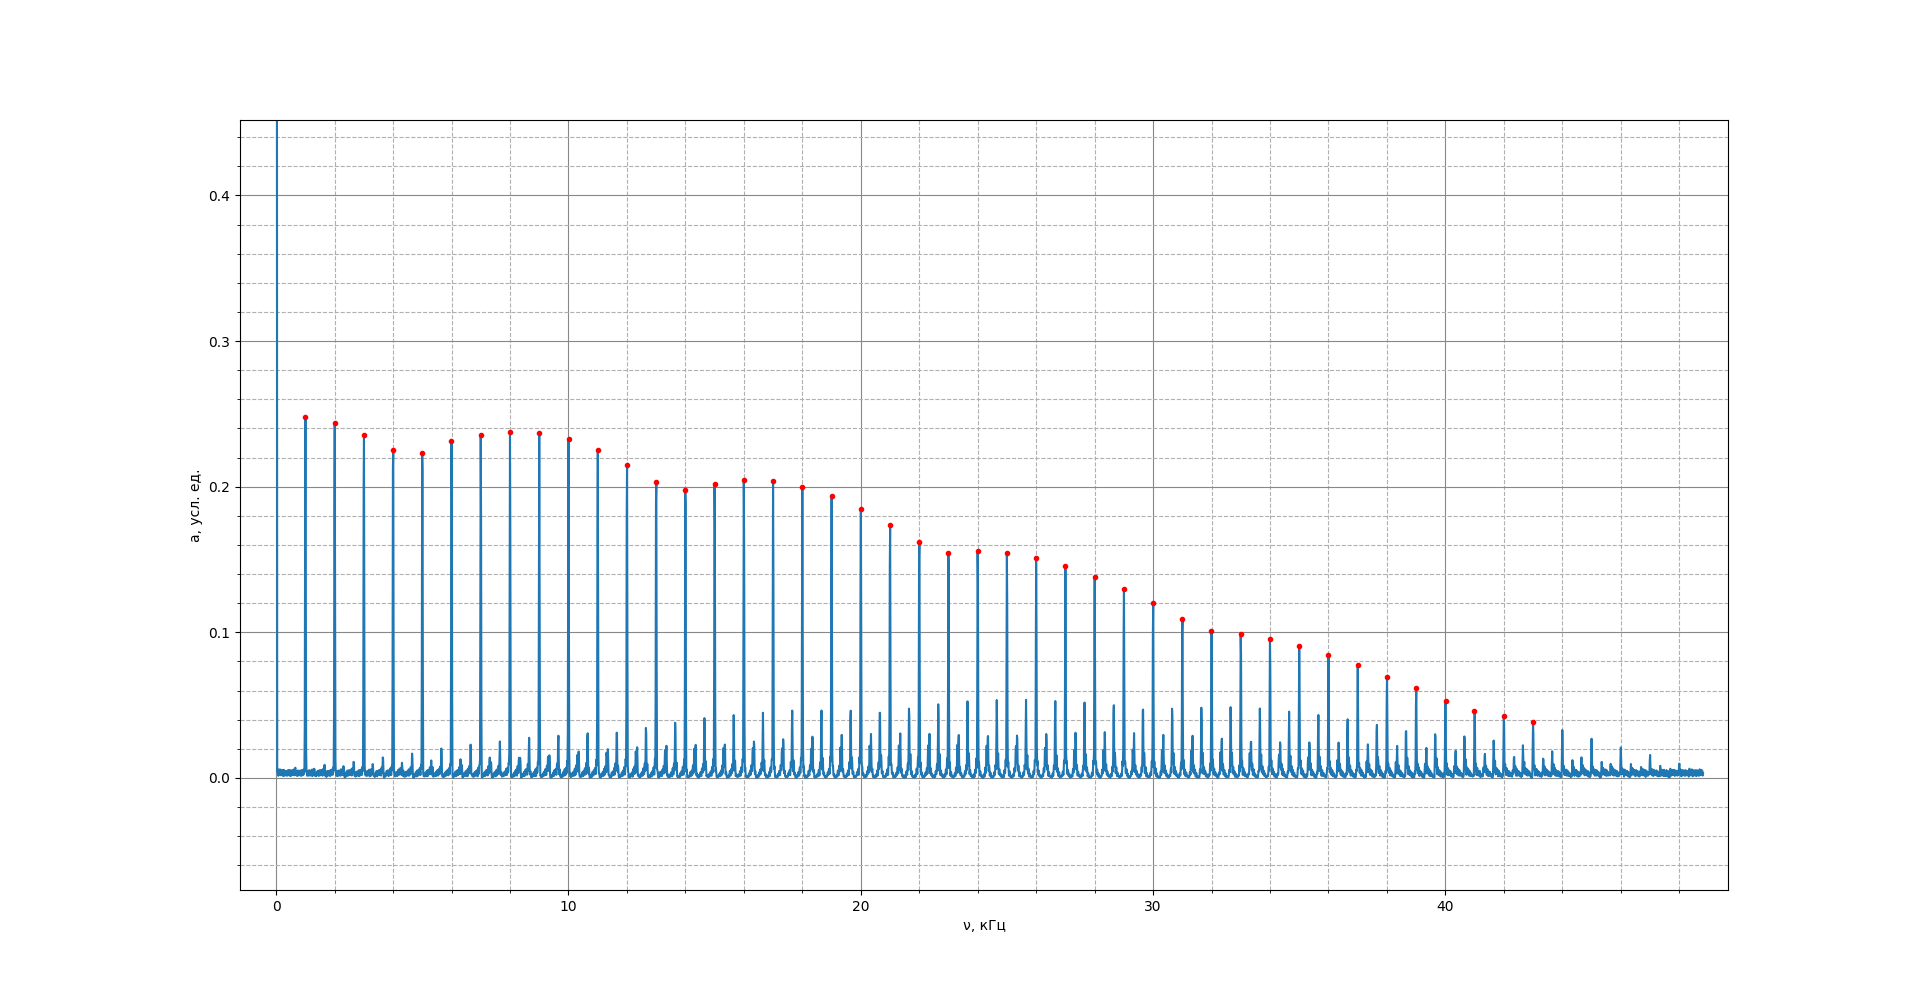
\includegraphics[width=0.5\textwidth]{20us.png}}}\\
    \subfloat[$\nu_{\text{повт}} = 1$ кГц, $\tau = 60$ мкс.]{{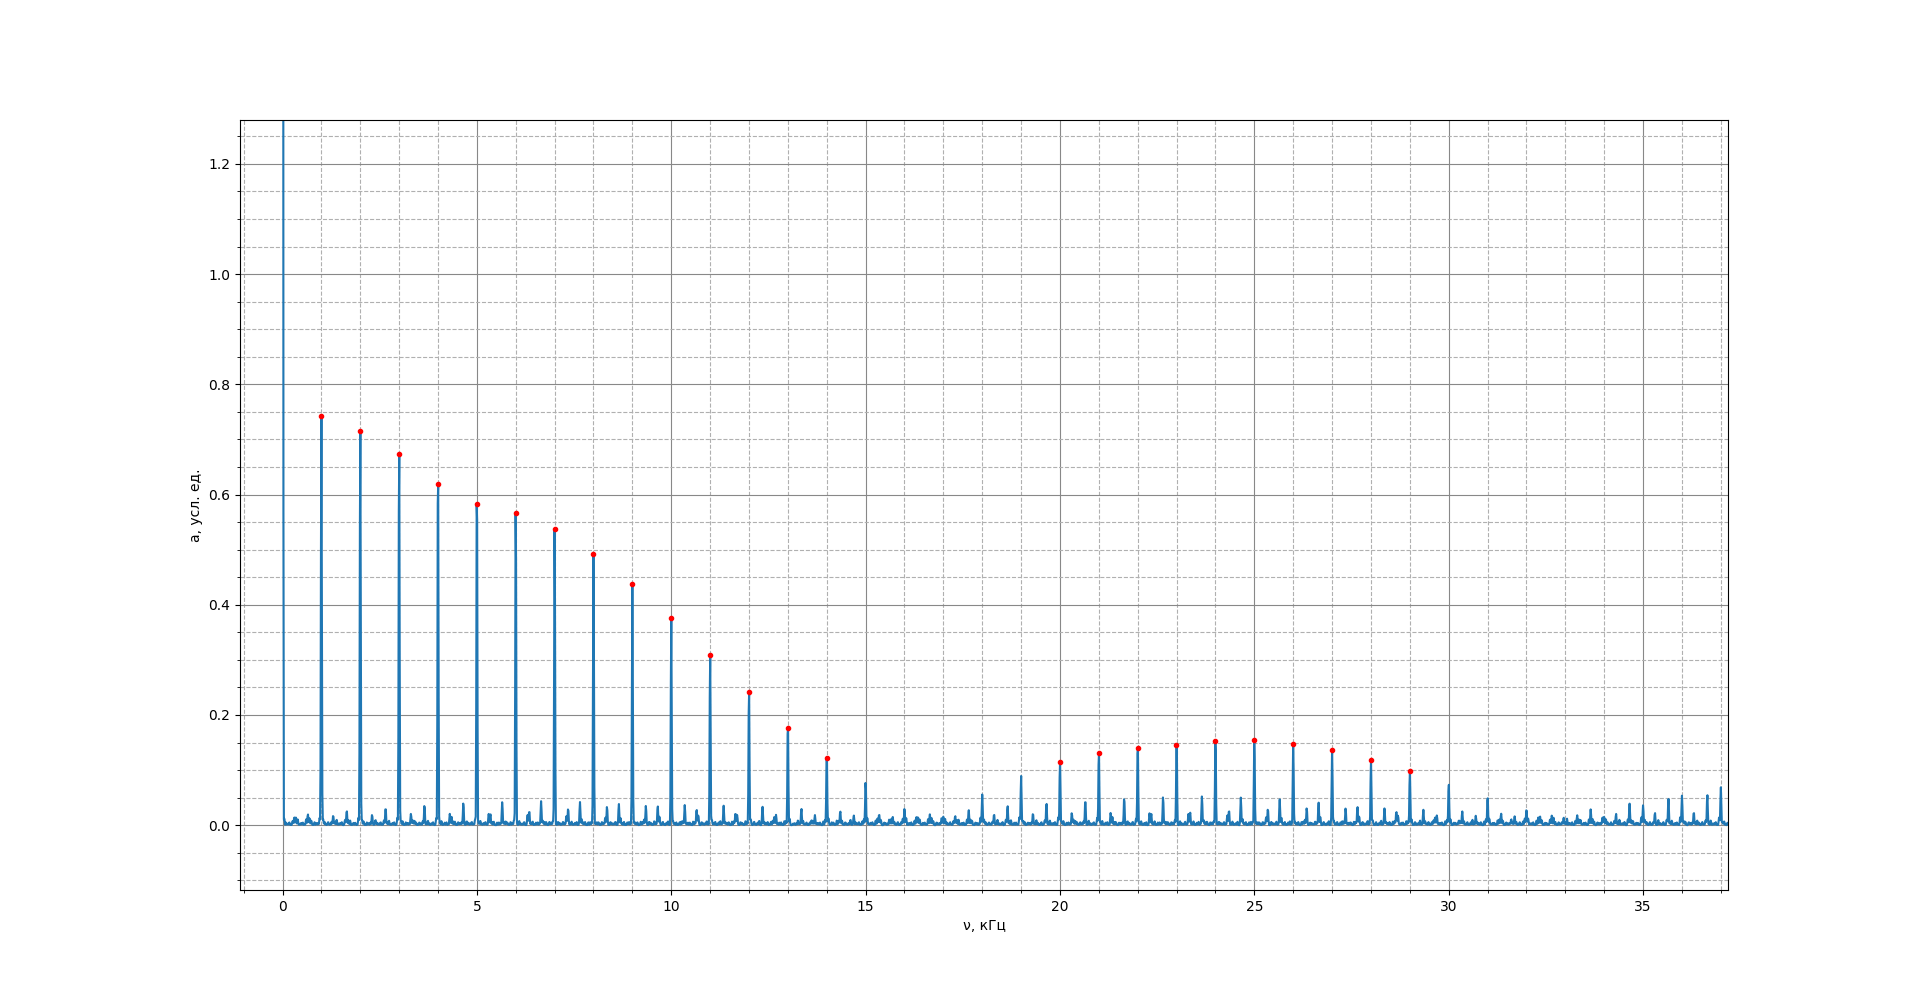
\includegraphics[width=0.5\textwidth]{60us.png}}}
    \subfloat[$\nu_{\text{повт}} = 1$ кГц, $\tau = 80$ мкс.]{{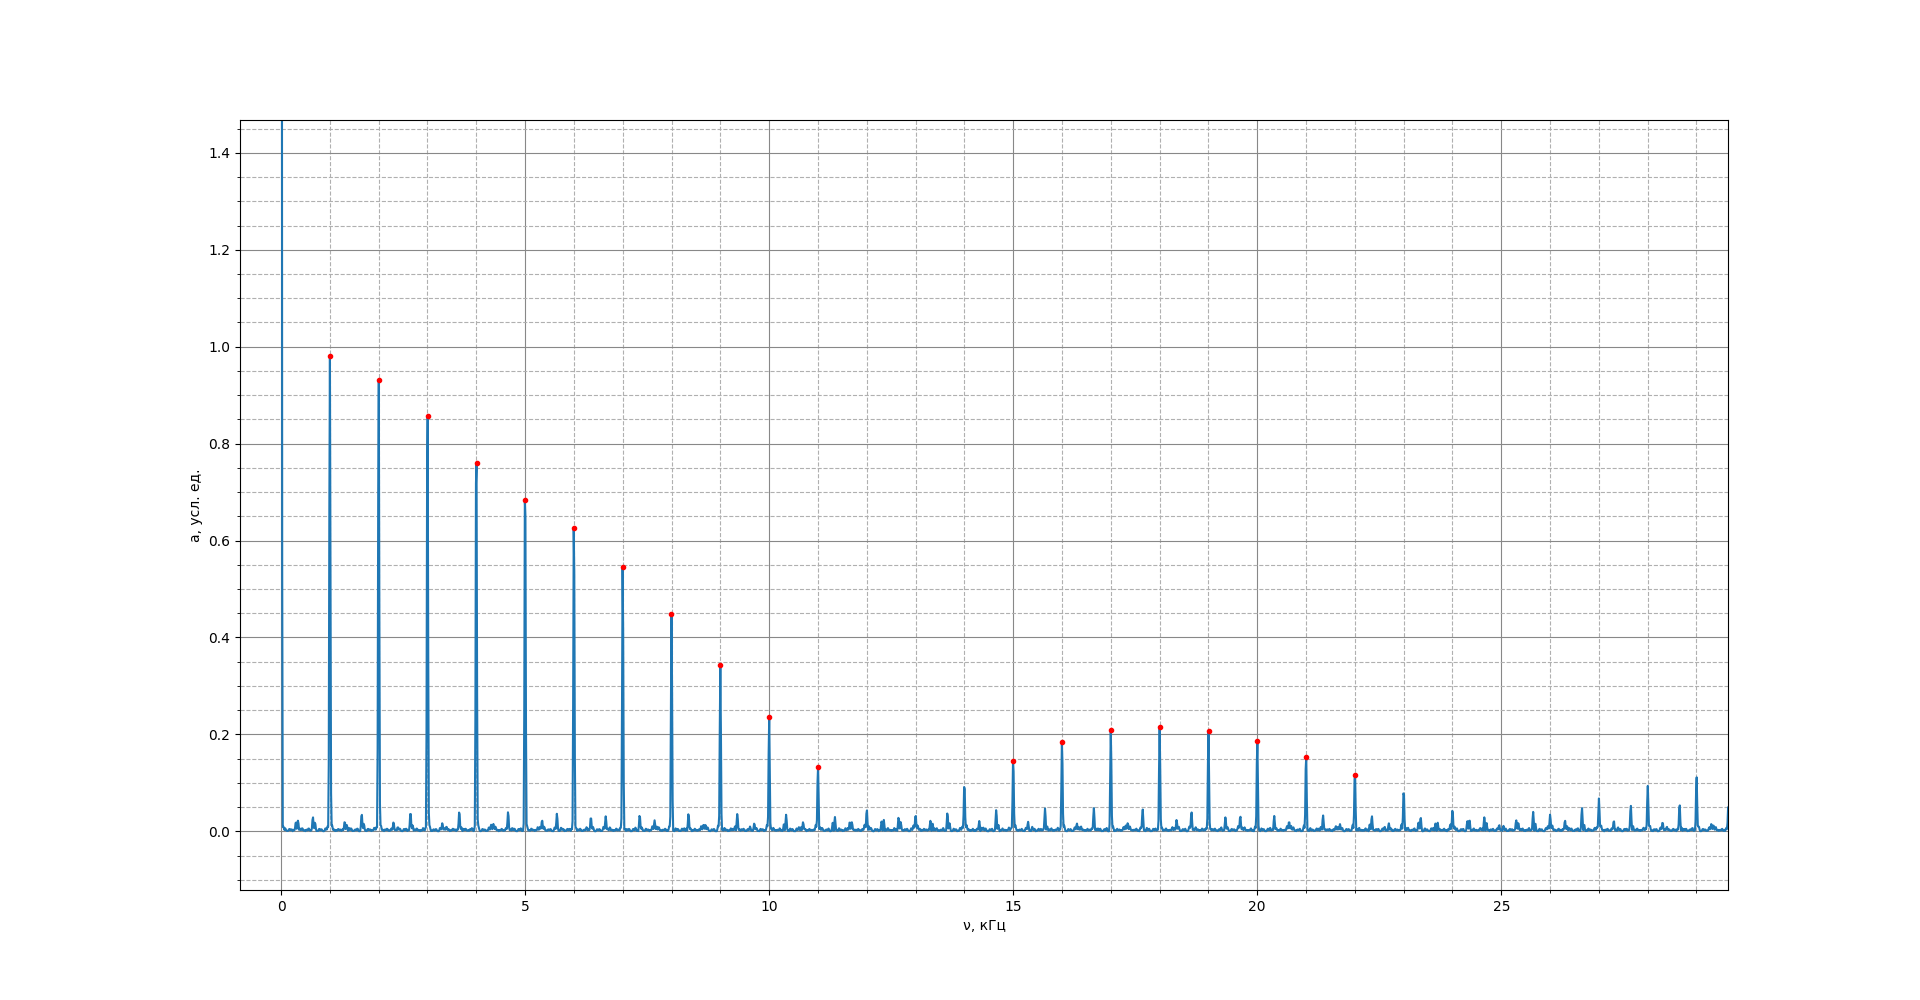
\includegraphics[width=0.5\textwidth]{80us.png}}}\\
    \subfloat[$\nu_{\text{повт}} = 1$ кГц, $\tau = 100$ мкс.]{{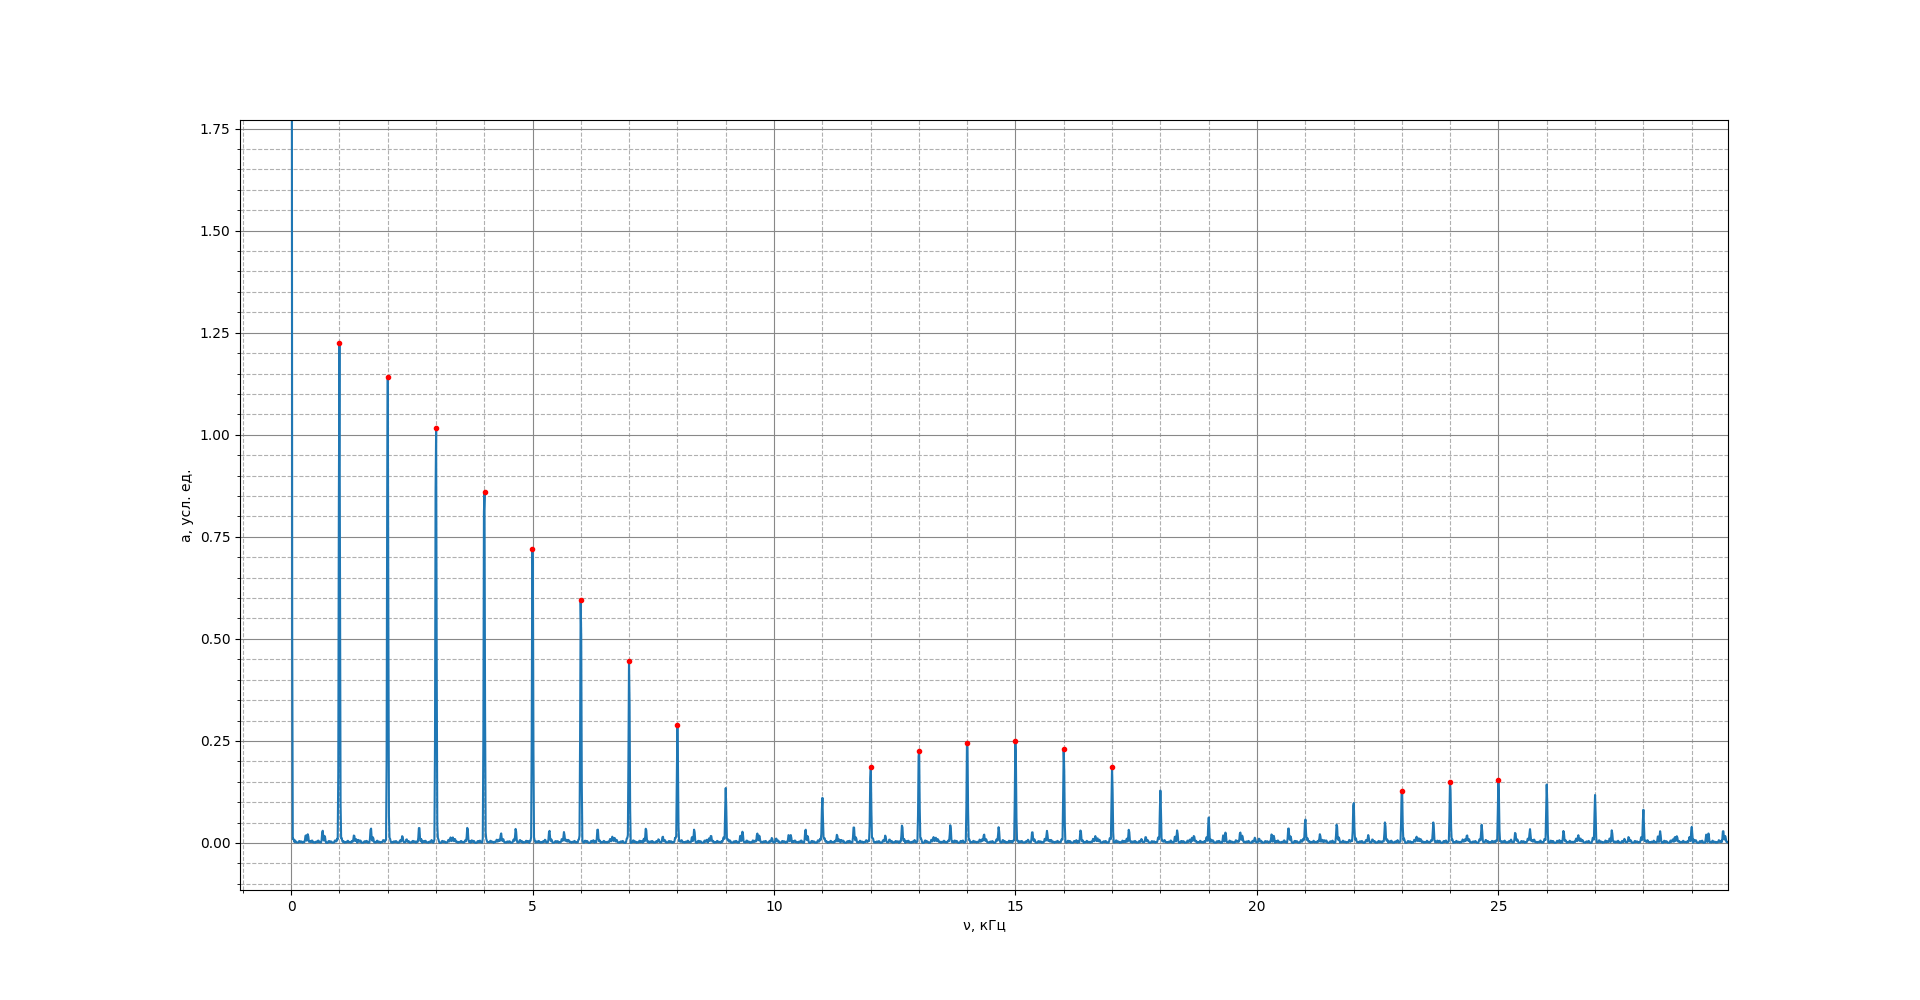
\includegraphics[width=0.5\textwidth]{100us.png}}}
    \subfloat[$\nu_{\text{повт}} = 1$ кГц, $\tau = 140$ мкс.]{{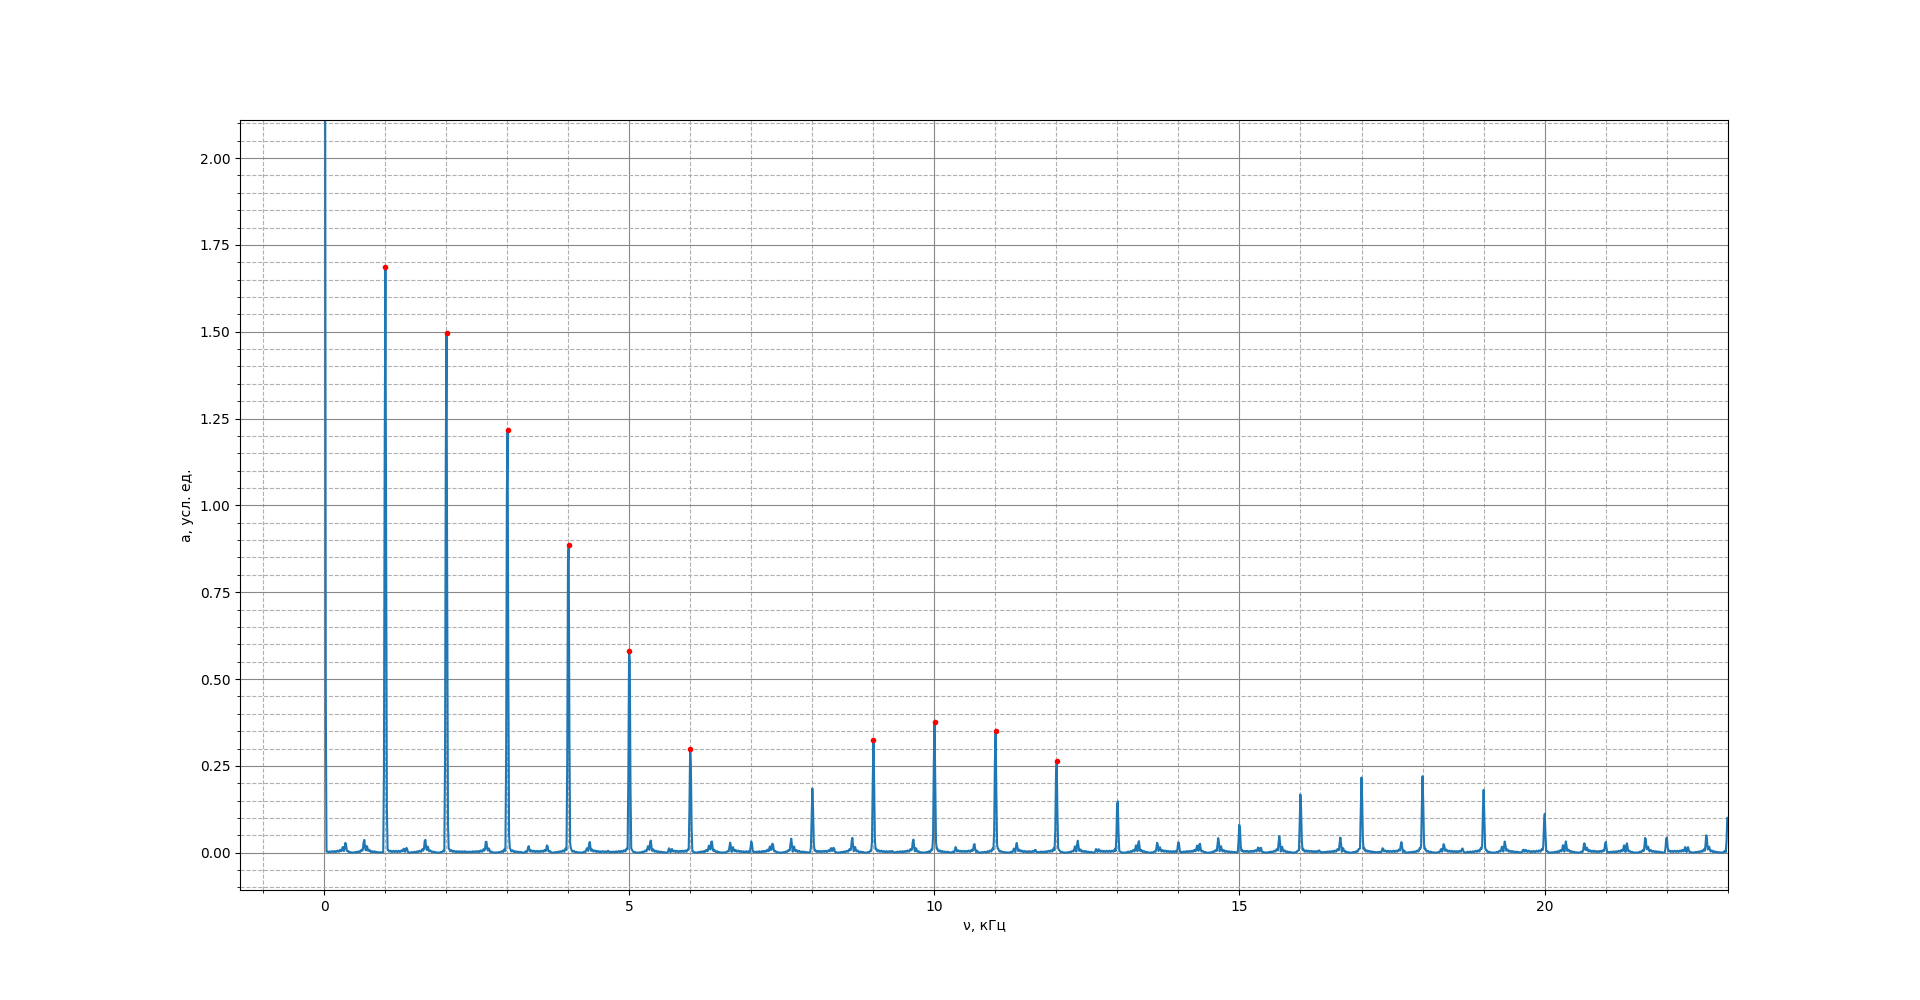
\includegraphics[width=0.5\textwidth]{140us.png}}}\\
    \subfloat[$\nu_{\text{повт}} = 1$ кГц, $\tau = 180$ мкс.]{{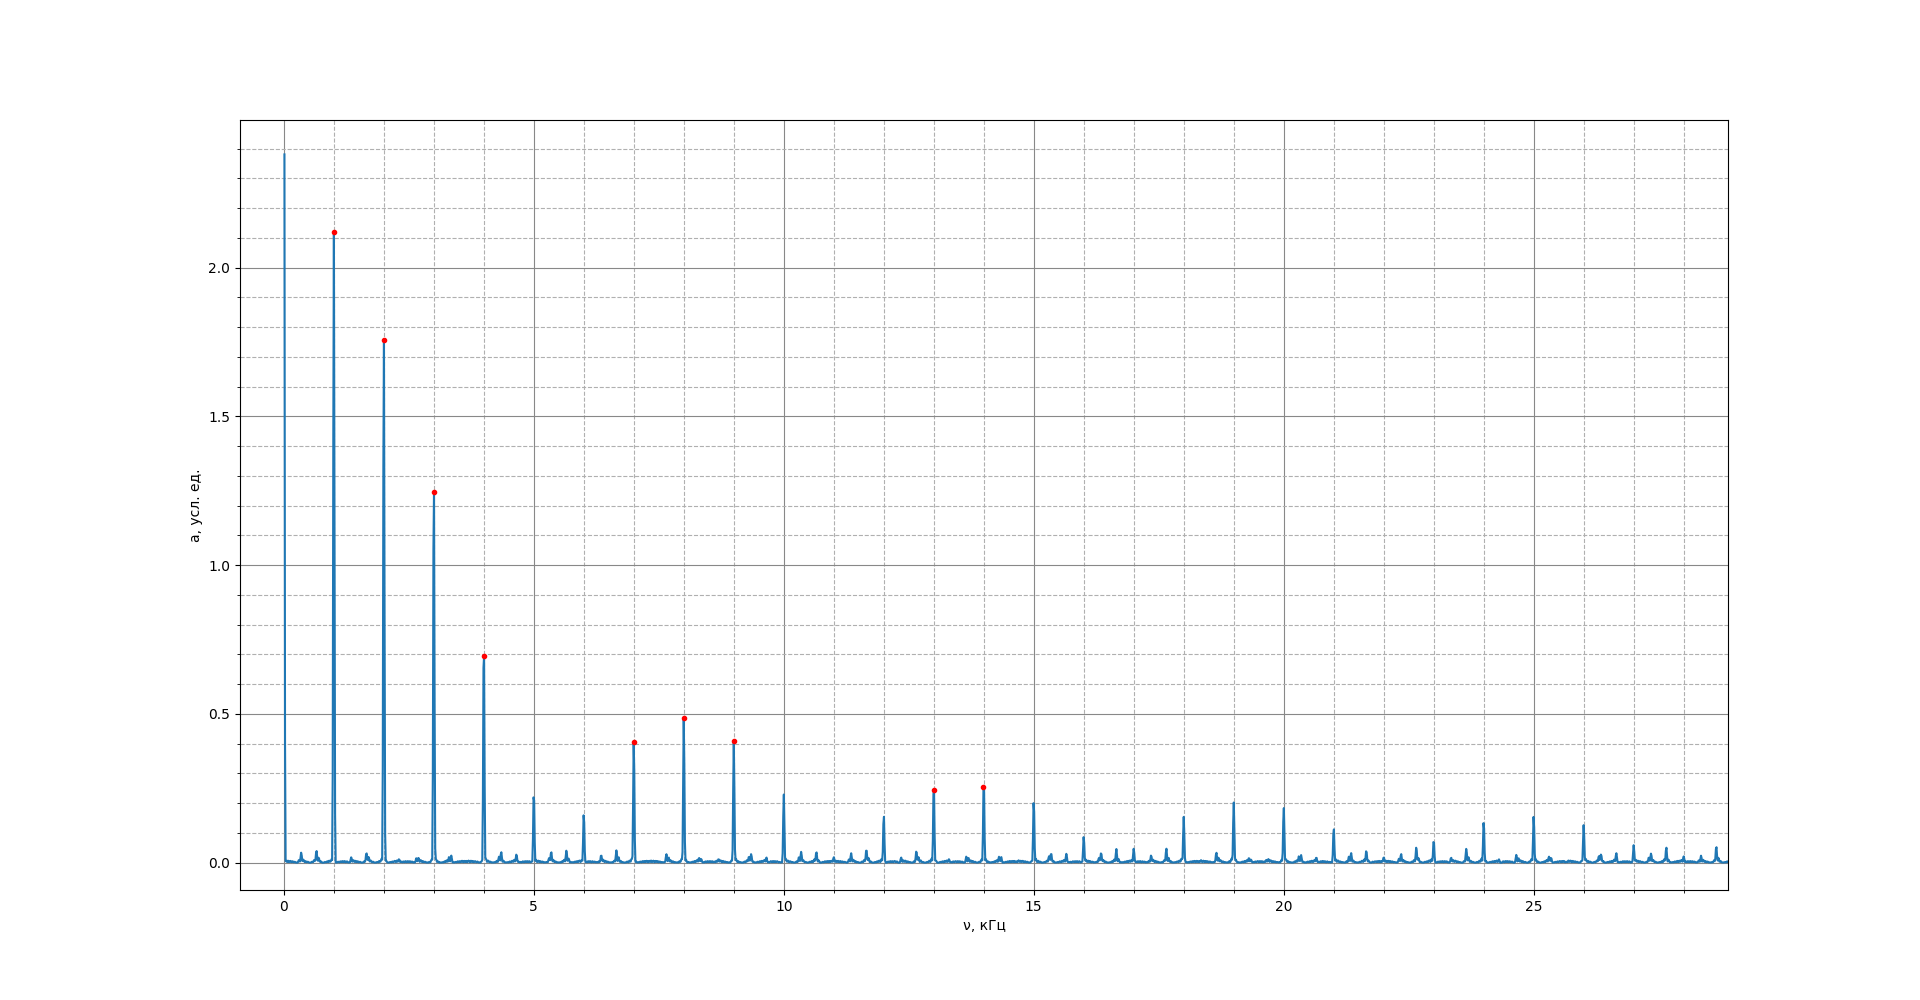
\includegraphics[width=0.5\textwidth]{180us.png}}}
\end{figure}

Затем зафиксировали $\nu_{\text{повт}} = 1$ кГц и $\tau = 60$ мкс. Для этих параметров измерили величину $a_n$ и $\nu_n$ для 13 гармоник и сравнили с рассчитанными значениями по формулам. Результаты занесли в таблицу.
\[\nu_n = \frac{n}{T} \]
\[|a_n| = \frac{|\sin{ \frac{\pi n \tau}{T}}|}{\pi n}\]


\begin{center}
\begin{tabular}{|l|l|l|l|l|l|l|l|l|l|l|l|l|l|}
\hline
n                        & 1    & 2    & 3    & 4    & 5    & 6    & 7    & 8    & 9    & 10    & 11    & 12    & 13    \\ \hline
$\nu_n^{exp}$            & 1.00 & 2.00 & 3.00 & 4.01 & 4.99 & 6.00 & 7.00 & 8.00 & 9.00 & 10.00 & 11.00 & 12.00 & 13.01 \\ \hline
$\nu_n^{theor}$          & 1    & 2    & 3    & 4    & 5    & 6    & 7    & 8    & 9    & 10    & 11    & 12    & 13    \\ \hline
$a_n^{exp}$              & 0.74 & 0.72 & 0.67 & 0.62 & 0.58 & 0.57 & 0.54 & 0.49 & 0.44 & 0.38  & 0.31  & 0.24  & 0.18  \\ \hline
$|a_n / a_1|^{exp}$      & 1    & 0.96 & 0.91 & 0.83 & 0.79 & 0.76 & 0.72 & 0.66 & 0.59 & 0.51  & 0.42  & 0.33  & 0.24  \\ \hline
$|a_n / a_1|^{theor}$    & 1    & 0.98 & 0.95 & 0.91 & 0.86 & 0.80 & 0.74 & 0.67 & 0.59 & 0.51  & 0.43  & 0.34  & 0.26  \\ \hline
\end{tabular}
\end{center}





\FloatBarrier

Далее зафиксировали период повторения T прямоугольного сигнала $T = 1мс$, $\nu_{\text{повт}} = 1кГц$. Изменяя длительность импульса $\tau$, измерили полную ширину спектра сигнала $\Delta \nu$. Полученные данные хаписали в таблице. Из таблицы легко заметить, что $\Delta \nu \tau \approx 1$, т.е. что выполняетсясоотношение неопределенностей.


\begin{center}
\begin{tabular}{|l|l|l|l|l|l|l|l|l|l|l|}
\hline
$\tau$, мкс                  & 20    		& 40    	   & 60    	      & 80    		 & 100             \\ \hline
$\Delta \nu$, кГц            & $46.48 \pm 0.58$ & $23.58 \pm 0.29$ & $15.60 \pm 0.14$ & $12.21 \pm 0.08$ & $9.73 \pm 0.07$ \\ \hline 
$\tau$, мкс		     & 120    		& 140    	   & 160    	      & 180    		 & 200             \\ \hline
$\Delta \nu$, кГц	     & $8.05 \pm 0.07$  & $6.80 \pm 0.07$  & $5.82 \pm 0.04$  & $5.04 \pm 0.02$  & $4.68 \pm 0.02$ \\ \hline
\end{tabular}
\end{center}


После этого мы зафиксировали длительность импульса $\tau = 100$ мкс. Изменяя частоту повторения $\nu_{\text{повт}}$, измерили расстояние $\delta \nu$ между соседними гармониками спектрами. Данные так же представлены в таблице.

\begin{center}
\begin{tabular}{|l|l|l|l|l|}
\hline
$\nu_{\text{повт}}$, Гц     & 200    	      & 500    		& 1000    	  & 2000             \\ \hline
$\delta \nu$, Гц            & $199.8 \pm 1.6$ & $499.9 \pm 1.5$ & $999.4 \pm 3.6$ & $1996.8 \pm 8.4$ \\ \hline
\end{tabular}
\end{center}

\FloatBarrier

\begin{figure}[h]
    \centering
    \subfloat[МНК для графика $\Delta \nu (1/\tau)$\\
	      коэффициент наклона $k = (92.8 \pm 1.0) 10^{-5}$]{{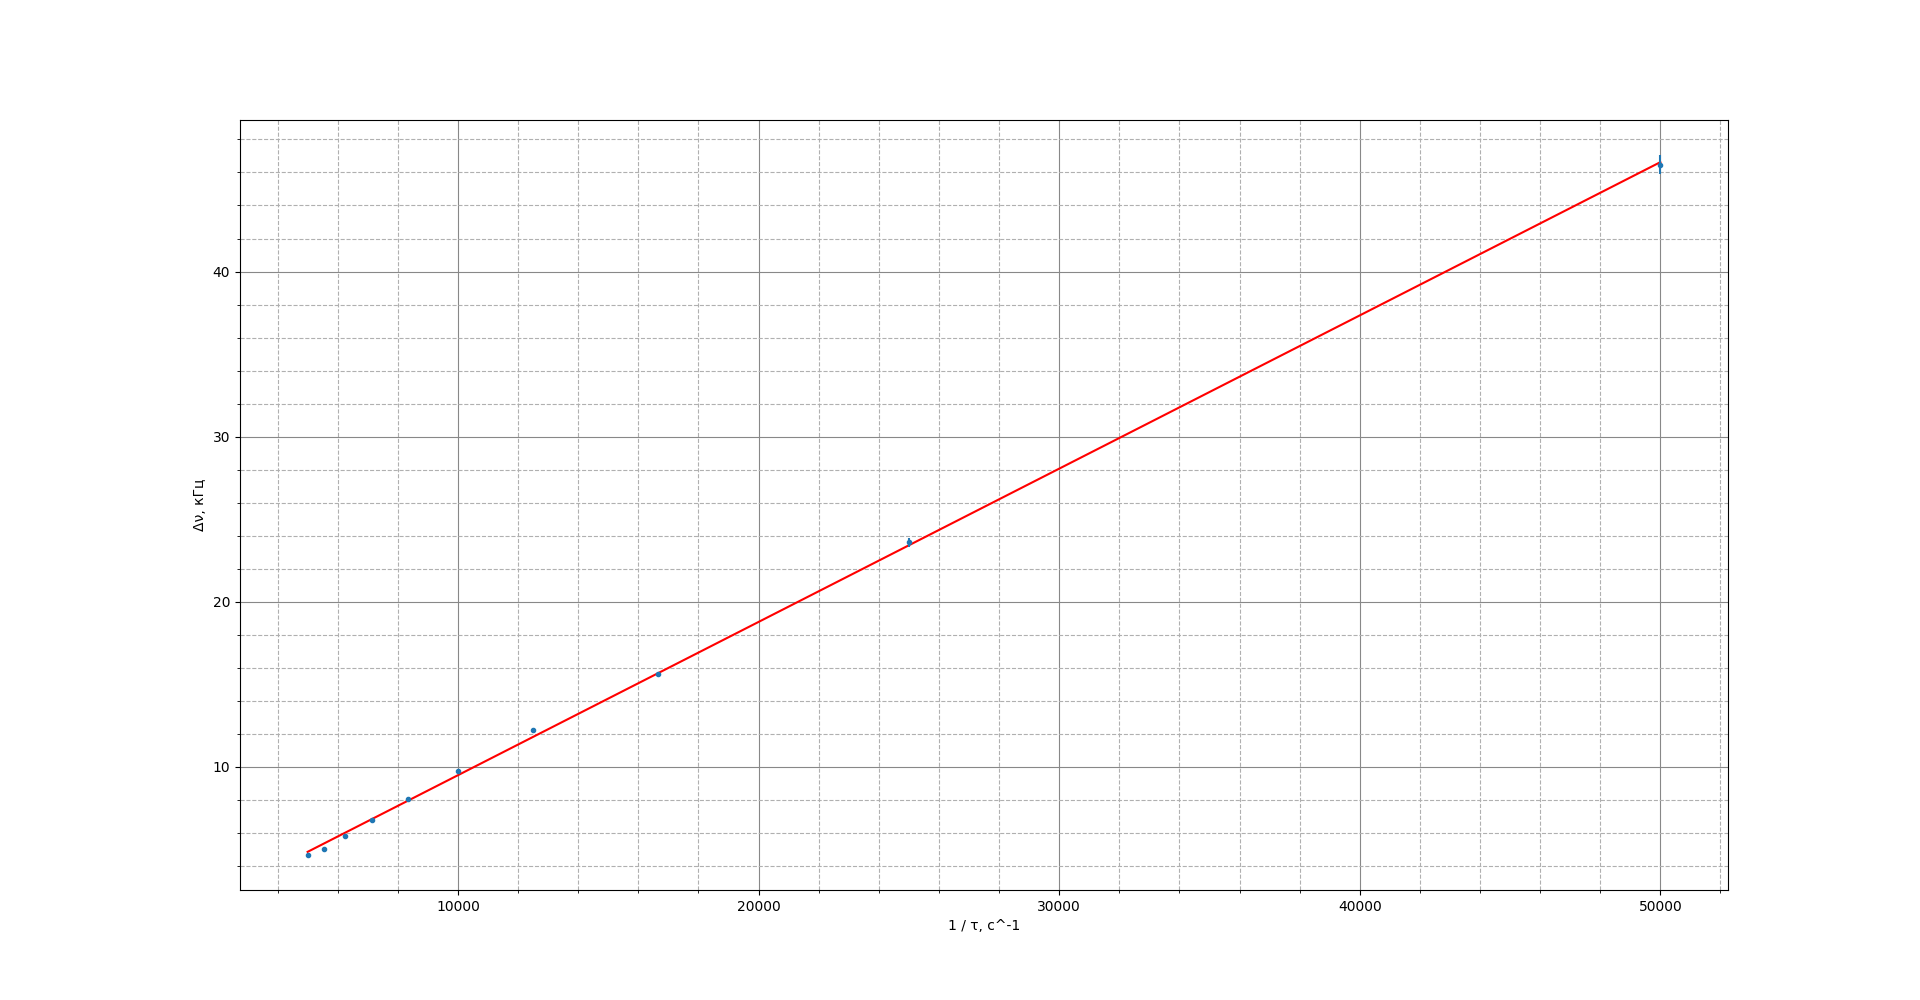
\includegraphics[width=0.5\textwidth]{lsqm tau.png}}}
    \subfloat[МНК для графика $\delta \nu (1/T)$\\
	      коэффициент наклона $k = (998.2 \pm 4.2) 10^{-6}$]{{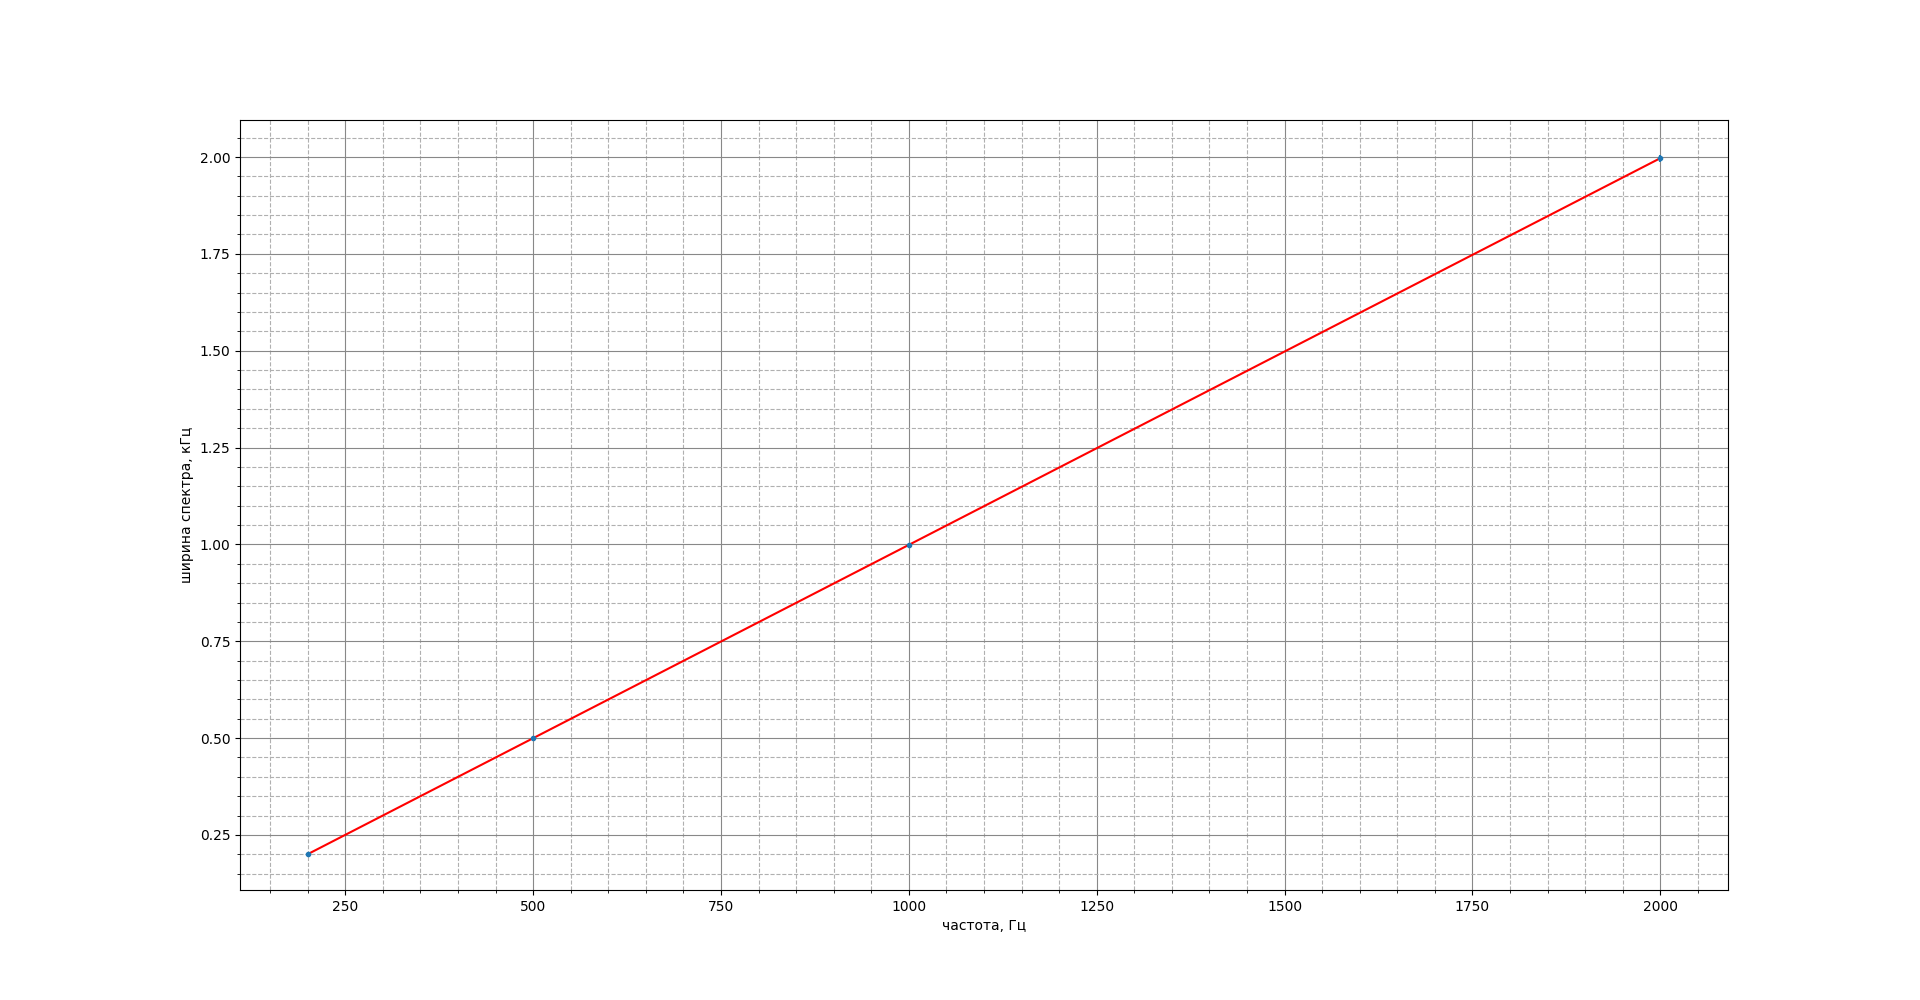
\includegraphics[width=0.5\textwidth]{lsqm T.png}}}\\
\end{figure}




\end{document}